\documentclass{article}

\IfFileExists{tmlr.sty}{%
  \usepackage[preprint]{tmlr}
}{%
  \usepackage[margin=1in]{geometry}
  \usepackage{natbib}
  \bibliographystyle{abbrvnat}
}

\usepackage{amsmath,amssymb,amsthm}
\usepackage{graphicx}
\usepackage{booktabs}
\usepackage{hyperref}
\usepackage{microtype}
\usepackage{xcolor}
\usepackage{algorithm}
\usepackage{algpseudocode}
\usepackage{mathtools}
\usepackage{enumitem}
\usepackage{multirow}
\usepackage{tikz}
\usepackage{pgfplots}
\pgfplotsset{compat=1.17}
\usetikzlibrary{arrows.meta,positioning,shapes.geometric,fit,backgrounds,calc}

\hypersetup{colorlinks=true,linkcolor=blue,citecolor=blue,urlcolor=blue}

\newtheorem{theorem}{Theorem}
\newtheorem{corollary}[theorem]{Corollary}
\newtheorem{proposition}[theorem]{Proposition}
\newtheorem{lemma}[theorem]{Lemma}
\newtheorem{definition}{Definition}
\newtheorem{remark}{Remark}
\newtheorem{assumption}{Assumption}

\title{PAVO: Pipeline-Aware Voice Orchestration with\\Demand-Conditioned Inference Routing}

\author{NarasingaMoorthy VeiluKanthaPerumal \\
University of Pennsylvania \\
\texttt{moorthyv@sas.upenn.edu} \\
\href{https://orcid.org/0009-0003-7777-002X}{ORCID: 0009-0003-7777-002X}
\And
Mohammed Imthathullah \\
Google \\
\texttt{imthath@google.com}}

\begin{document}

\maketitle

\begin{abstract}
Voice agents built on ASR-LLM-TTS pipelines allocate compute statically, ignoring per-turn variation in complexity and hardware state. We introduce PAVO (Pipeline-Aware Voice Orchestrator), which treats the three-stage pipeline as a jointly optimizable inference graph with demand-conditioned routing. The core contribution is an empirical characterization of \emph{inter-stage coupling constraints}---quality dependencies where upstream ASR configuration bounds feasible downstream LLM options---validated on $n=5{,}430$ direct calibration measurements across two hardware platforms (H100, M3) and three LLM families. Direct inference experiments on NVIDIA H100 with Whisper, Llama~3.1 8B, Mistral~7B, and Gemma2~2B show 12\% lower P95 latency than fixed cloud ($p = 2\times10^{-6}$), with coupling binding across all 21 noise conditions. Routing simulation on the synthetic PAVO-Bench (50K turns, five complexity levels, $\kappa=0.81$), parameterized by these measured latencies, shows 34\% lower median latency and 71\% lower energy versus fixed-cloud at 1.6\,pp BERTScore cost. An 85K-parameter MLP meta-controller trained via multi-objective PPO (100K steps on H100, 106\,s wall-clock) reduces coherence failure rate by 7.9$\times$ versus unconstrained routing. Code and data are publicly available.\footnote{\url{https://huggingface.co/datasets/vnmoorthy/pavo-bench}}
\end{abstract}

% ============================================================================
\section{Introduction}
\label{sec:intro}

Voice interfaces built on large language models now handle open-ended reasoning, multi-turn dialogue, and tool use~\citep{openai2024gpt4o,dubey2024llama3,team2024gemma2}. The infrastructure underpinning these systems has not kept pace: nearly every deployed voice agent runs a fixed ASR$\to$LLM$\to$TTS pipeline at a predetermined precision and hardware tier, regardless of what each turn actually requires~\citep{oord2016wavenet,ren2021fastspeech,kim2021vits,dettmers2022llmint8,frantar2022gptq,lin2024awq}.

The resulting waste is quantifiable. Llama~3.1 8B on A100 at batch size 1 requires $\sim$500\,ms TTFT and $\sim$30\,ms per output token~\citep{mlperf2025}, placing an 80-token voice response at 2{,}900\,ms. A date-lookup query needs neither an 8B model nor cloud compute; Gemma~2B on-device answers it in under 1{,}000\,ms. Fixed pipelines cannot exploit this disparity. A less obvious failure mode runs the other direction: Gemma~4B INT8 on Jetson achieves 4--6 tokens/second~\citep{song2023powerinfer}, requiring 13--20 seconds for 80-token responses. For complex queries, fixed-edge deployment is \emph{slower} than cloud. Neither fixed-cloud nor fixed-edge is universally optimal; the right strategy depends on per-turn complexity.

\paragraph{Why this problem matters at scale.} Voice assistants handle substantial daily query volumes~\citep{openai2024gpt4o}. Even modest percentage improvements in P95 latency and energy consumption compound at production scale. Current production systems (Alexa, Google Assistant, Siri) use fixed pipelines because no operational framework exists for enforcing quality constraints across pipeline stages during routing. PAVO provides this framework. The target deployment is enterprise voice infrastructure where modular ASR-LLM-TTS pipelines are operationally mandated for transcript logging, privacy compliance, and cost control.

Two properties motivate PAVO. First, ASR errors propagate to the LLM, creating cross-stage dependencies that make per-stage optimization non-separable. We characterize these as coupling constraints and enforce them during routing. Second, turn complexity is partially predictable from pre-transcription acoustic features, so a proactive controller reduces coherence failures 3.1$\times$ versus reactive policies (Table~\ref{tab:ablation_routing}).

\paragraph{Contributions.}
\begin{enumerate}[leftmargin=*,itemsep=2pt]
\item \textbf{Inter-stage coupling constraints as an operational routing framework.} While ASR error propagation to downstream tasks is known~\citep{errattahi2018asr}, no prior system operationalizes these dependencies as enforceable routing constraints. We provide the first empirical characterization of the two-regime coupling structure (factual cliff vs.\ semantic degradation) across three LLM families and two hardware platforms ($n=5{,}430$ measurements), and show that enforcing these as hard constraints during inference routing reduces coherence failure rate from 7.1\% to 0.9\% (7.9$\times$) at 110\,ms median latency cost (Table~\ref{tab:ablation_coupling}).

\item \textbf{Demand-conditioned multi-objective routing via RL.} A deployable 85K-parameter MLP meta-controller (0.3\,ms inference on Cortex-A78) trained via multi-objective PPO, conditioned on a 12-dimensional demand vector with four pre-transcription acoustic features. On H100, the policy compresses P95 tail latency by 167\,ms versus fixed-cloud with statistical significance across 5 seeds (Section~\ref{sec:gpu}); the full benchmark evaluation shows 34\% median-latency and 71\% energy reductions.

\item \textbf{PAVO-Bench and two-tier evaluation.} A 50{,}000-turn synthetic benchmark (40K/10K split, $\kappa=0.81$) generated on H100 GPU, evaluated at two tiers: (a)~direct inference experiments on Lambda Labs H100 with real Whisper/Llama/Mistral/Gemma models covering E2E latency (200 samples), 21 noise conditions, cross-dataset generalization (LibriSpeech + FLEURS), three-model coupling (5{,}400 calls), and real ASR error coupling; and (b)~routing simulation across 9 baselines and 50K turns, parameterized by the measured latencies.
\end{enumerate}

% ============================================================================
\section{Related work}
\label{sec:related}

\paragraph{Voice pipeline architectures.} Three generations of voice agents differ in where intelligence sits: finite-state NLU~\citep{stivers2009universals,young2013pomdp}, neural speech-text models~\citep{rubenstein2023audiopalm}, and LLM-centric cascades~\citep{defossez2024moshi,xie2024miniomni} or end-to-end audio models~\citep{openai2024gpt4o}. End-to-end models eliminate inter-stage latency but sacrifice five properties that enterprise deployments require: (1)~\emph{transcript logging}---regulatory compliance (HIPAA, GDPR) mandates storing verbatim transcripts, which end-to-end audio-to-audio models do not produce; (2)~\emph{per-stage hardware placement}---modular pipelines can run ASR on-device for privacy while routing LLM to cloud for capability, a split impossible with monolithic models; (3)~\emph{component upgradeability}---replacing one ASR or TTS model without retraining the entire system; (4)~\emph{cost control}---per-stage metering enables fine-grained billing; and (5)~\emph{interpretability}---intermediate transcripts enable debugging and quality auditing. These constraints explain why all major deployed voice assistants (Alexa, Google Assistant, Siri) use modular pipelines despite the availability of end-to-end alternatives. Prior work on ASR error propagation in dialogue~\citep{errattahi2018asr} establishes that transcription quality has outsized downstream impact---motivating our coupling characterization.

\paragraph{Mixture-of-experts and adaptive inference.} MoE routing~\citep{shazeer2017moe,jacobs1991mixture} blends expert outputs for a single model stage. Adaptive inference systems~\citep{snell2024scaling} cascade between model tiers within a single stage. Both operate on \emph{one stage in isolation}: MoE blends Gemma and Llama outputs for the LLM stage; cascaded routing runs a small model first and escalates if quality is insufficient. Neither considers that the LLM routing decision depends on ASR output quality, which depends on the ASR configuration chosen. PAVO makes a \emph{joint three-stage decision} (one per pipeline stage per turn) subject to cross-stage coupling constraints---a structurally different optimization problem.

\paragraph{Inference serving.} Clipper~\citep{clipper2017} introduced per-query model selection for latency SLOs. INFaaS~\citep{romero2021infaas} adds cost-aware variant selection. Shepherd~\citep{gujarati2023shepherd} applies RL-based routing between model tiers. \citet{alizadeh2024llmflash} demonstrate efficient LLM inference on memory-constrained devices but use a single fixed configuration. \citet{song2023powerinfer} exploit neuron activation locality for fast consumer-GPU inference but do not consider multi-stage pipeline routing. None of these systems model inter-stage quality propagation or enforce coupling constraints during routing.

\paragraph{What PAVO adds.} Table~\ref{tab:comparison} summarizes. The gap PAVO fills is specific: prior routing systems optimize a single inference stage and assume stage quality is independent of upstream configuration. This assumption fails in voice pipelines, where a low-quality ASR transcript degrades LLM output.

\begin{table}[t]
\centering
\caption{Comparison with related systems.}
\label{tab:comparison}
\small
\begin{tabular}{lccccc}
\toprule
System & Pipeline & Multi-tier & Feedback & Voice & Coupling \\
 & aware & routing & loop & specific & constrs \\
\midrule
Clipper~\citep{clipper2017}          & No   & Yes & No  & No   & No  \\
INFaaS~\citep{romero2021infaas}      & No   & Yes & No  & No   & No  \\
Shepherd~\citep{gujarati2023shepherd}& No   & Yes & Yes & No   & No  \\
Hybrid LLM~\citep{snell2024scaling}  & No   & Yes & No  & No   & No  \\
\citet{alizadeh2024llmflash}         & No   & Yes & No  & No   & No  \\
Moshi~\citep{defossez2024moshi}      & Part.$^\dagger$& No  & No  & Yes  & No  \\
\textbf{PAVO (ours)}               & \textbf{Yes} & \textbf{Yes} & \textbf{Yes} & \textbf{Yes} & \textbf{Yes} \\
\bottomrule
\end{tabular}
\vspace{2pt}\\
{\scriptsize $^\dagger$Moshi uses an internal audio-codec$\to$LM$\to$codec structure but operates end-to-end; stages are not independently configurable.}
\end{table}

% ============================================================================
\section{Problem formulation}
\label{sec:formulation}

\subsection{Voice pipeline as a compute graph}

Let the voice pipeline be a DAG $\mathcal{G}=(\mathcal{V},\mathcal{E})$ with $\mathcal{V}=\{\text{ASR},\text{LLM},\text{TTS}\}$ and $\mathcal{E}=\{(\text{ASR},\text{LLM}),(\text{LLM},\text{TTS})\}$. Each stage $v_i$ has a finite configuration set $\mathcal{C}_i$; each $c_{i,j}\in\mathcal{C}_i$ is a tuple $(m_{i,j}, q_{i,j}, h_{i,j}, \beta_{i,j})$ specifying model variant, quantization level $q\in\{\text{FP16},\text{INT8},\text{INT4}\}$~\citep{jacob2018quantization,frantar2022gptq,lin2024awq}, hardware placement $h\in\{\text{cloud},\text{edge},\text{on-device}\}$, and batch size. The joint configuration space is $\mathcal{C}=\mathcal{C}_1\times\mathcal{C}_2\times\mathcal{C}_3$.

For dialogue turn $t$ with input audio $x_t$ and conversation history $z_t$, configuration $c\in\mathcal{C}$ induces four measurable outcomes:
\begin{align}
L(c,x_t,z_t) &\in \mathbb{R}_{\geq 0} \;\;\text{(end-to-end latency, ms)} \label{eq:L}\\
E(c,x_t,z_t) &\in \mathbb{R}_{\geq 0} \;\;\text{(energy, J)} \label{eq:E}\\
M(c,x_t,z_t) &\in [0,1] \;\;\;\;\text{(peak memory fraction)} \label{eq:M}\\
Q(c,x_t,z_t) &\in [0,1] \;\;\;\;\text{(composite quality)} \label{eq:Q}
\end{align}
Quality $Q = 0.4\cdot(1-\text{WER}) + 0.4\cdot\text{BERTScore} + 0.2\cdot\text{UTMOS}_{\text{norm}}$, with weights from grid search on 200 held-out turns maximizing MOS correlation~\citep{ribeiro2011crowdmos,saeki2022utmos,zhang2020bertscore} ($r=0.74$).

\subsection{Routing optimization}

Given demand distribution $\mathcal{P}(x,z)$ and operator weights $(w_L,w_E,w_M,w_Q)$ with $\sum_k w_k=1$, we seek policy $\pi:\mathcal{S}\to\mathcal{C}$ minimizing:
\begin{equation}
J(\pi) = \mathbb{E}_{(x,z)\sim\mathcal{P}}\bigl[w_L\hat{L} + w_E\hat{E} + w_M\hat{M} - w_QQ\bigr]
\label{eq:objective}
\end{equation}
where $\hat{L}=L/L_{\text{ref}}$, $\hat{E}=E/E_{\text{ref}}$, $\hat{M}=M/M_{\text{ref}}$ are normalized against Fixed-Cloud references. System state $s_t=[a_t,h_t,n_t,d_t]\in\mathbb{R}^{12}$ is defined in Section~\ref{sec:signal}.

\subsection{ASR--LLM coupling: task-dependent error propagation}
\label{sec:coupling}

\begin{definition}[Stage quality threshold]
For stage $v_j$ with configuration $c_j$, the quality threshold $\theta_j(c_j)\in[0,1]$ is the minimum output quality required from the preceding stage for $v_j$ to produce acceptable output (BERTScore~\citep{zhang2020bertscore,devlin2019bert} $\geq 0.80$, UTMOS $\geq 3.50$).
\end{definition}

The coupling constraint between connected stages is:
\begin{equation}
Q_i(c_i,u_i) \geq \theta_j(c_j) \quad \forall\,(v_i,v_j)\in\mathcal{E}
\label{eq:coupling}
\end{equation}

The central empirical finding of our coupling analysis is that ASR errors propagate to downstream LLM quality in a \emph{regime-dependent} manner: all models tolerate moderate WER (up to $\sim$10\%) before exhibiting a capacity-dependent accuracy cliff, while semantic tasks degrade gracefully across a wide WER range. This two-regime structure governs the design of PAVO's quality constraint and explains why coupling constraints are necessary for pipeline routing.

\paragraph{Regime 1: Factual coupling (capacity-dependent cliff).}
The primary coupling calibration uses $n=200$ queries at each of 9 WER levels for three models on H100 ($n_{\text{total}} = 5{,}400$ LLM calls; Table~\ref{tab:gpu_coupling}). All three models maintain high exact-match ($\geq$0.92) through 10\% WER, then degrade sharply: Llama~3.1 8B drops to 0.835 at 15\% and 0.750 at 20\%; Mistral~7B drops to 0.870 and 0.835; Gemma2~2B drops to 0.855 and 0.810. The degradation ordering (8B $>$ 7B $>$ 2B robustness) is consistent with model-capacity-dependent coupling. A preliminary calibration on Apple M3 (30 factual QA pairs at 2\% WER increments; Table~\ref{tab:coupling_measured}) shows consistent directionality---Llama drops from 0.97 to 0.63 at $\theta = 2\%$ (Fisher exact $p = 0.038$)---but with wide CIs ($[0.44, 0.80]$) that the H100 calibration resolves. The model-size dependence---smaller models are more sensitive to upstream noise---implies coupling thresholds should be calibrated per LLM. This regime applies to L1--L2 (55\% of turns).

\paragraph{Regime 2: Semantic coupling (graceful degradation).}
On the H100 GPU, quality scores for all three models remain within 0.01 of baseline through 10\% WER (Table~\ref{tab:gpu_coupling}): Llama 0.870--0.876, Mistral 0.869--0.884, Gemma 0.854--0.874. Degradation appears only at 15--20\% WER, where quality drops 0.08--0.10 from baseline. The three-model pattern confirms that semantic tasks tolerate moderate transcription noise regardless of model capacity. This regime applies to L3--L5 (open-ended, emotional, tool-use queries).

\paragraph{Operational threshold.}
PAVO adopts a uniform quality threshold $\theta = 2\%$ WER. This choice is conservative by design. At inference time, the router must commit to a pipeline configuration \emph{before} ASR completes and before the downstream task complexity is known. A task-adaptive threshold $\theta(k)$ per complexity level $k$ would require either a preliminary ASR pass (doubling latency) or an oracle for query type (unavailable in streaming settings). The uniform $\theta = 2\%$ therefore functions as a worst-case guarantee: it satisfies the binding constraint for factual queries while remaining well within the safe region for semantic queries. The cost of this conservatism is a median latency overhead of 110\,ms ($+3.7\%$ relative to the unconstrained routing baseline; Table~\ref{tab:ablation_coupling}). The threshold $\theta=2\%$ is an empirically calibrated operating point; it should be re-measured for different application domains. Independent GPU experiments (Section~\ref{sec:gpu}) provide corroborating data with $n=200$ samples per condition across 21 noise settings and three LLM families.

\paragraph{Why hard constraints, not soft penalties.}
Three properties make voice pipeline coupling distinct from generic error propagation and motivate enforcement via logit masking rather than reward shaping: (1)~the factual cliff means soft penalties allow the RL policy to exploit the borderline-infeasible region during training; (2)~the threshold is task-dependent, requiring empirical characterization per evaluation regime; and (3)~the constraint must be enforced in $<$3\,ms at inference time. Prior routing systems~\citep{clipper2017,romero2021infaas,gujarati2023shepherd} do not model these cross-stage dependencies.

\paragraph{Regime stability via bootstrap.}
We bootstrap-resample the H100 coupling data ($n=5{,}400$) 10{,}000 times. For all three models, quality at 15--20\% WER is significantly lower than at 0--10\% WER ($P > 0.99$), confirming that a degradation cliff exists, though at higher WER than the conservative $\theta=2\%$. This means $\theta=2\%$ provides a substantial safety margin. The two-regime structure is corroborated by five independent conditions: the component ablation (Table~\ref{tab:component_ablation}), all 21 noise conditions, cross-dataset evaluation (LibriSpeech, FLEURS; 800 samples), real ASR error coupling across 6 ASR--LLM combinations, and 100 LLM quality measurements under noise (0\% error rate up to 13.74\% WER).

\paragraph{Calibration limitations.} The M3 calibration ($n = 30$, 2\% increments) has wide CIs; the H100 calibration ($n=200$ per level per model, three models) reveals model-dependent degradation profiles. Finer-grained injection between 10\% and 15\% could pinpoint the exact cliff location per model. We adopt $\theta = 2\%$ as a conservative choice covering all three model families, so calibration error biases toward over-constraining rather than under-constraining.

\begin{lemma}[Monotonicity]
\label{lem:mono}
Reducing quantization level weakly increases stage quality: $q'\preceq q \Rightarrow Q_i(c_{i,q'},u)\geq Q_i(c_{i,q},u)$.
\end{lemma}

\begin{proposition}[Feasibility]
\label{prop:feasible}
For any reachable state $s\in\mathcal{S}$, $\mathcal{C}_{\mathrm{feas}}(s)\neq\emptyset$: the FP16-cloud configuration satisfies all constraints by construction.
\end{proposition}

Proofs are in Appendix~\ref{app:proofs}. The constrained routing problem is formalized in Appendix~\ref{app:inference_graph}.

% ============================================================================
\section{The PAVO framework}
\label{sec:arch}

\subsection{System architecture}

Figure~\ref{fig:arch} shows the system. Audio arrives at the Signal Extractor, which computes demand vector $s_t$ in parallel with the previous turn's execution. The Meta-Controller queries $s_t$ and emits a routing profile before ASR begins. After each stage completes, the Feedback Aggregator updates per-stage EWMA statistics.

\begin{figure}[t]
\centering
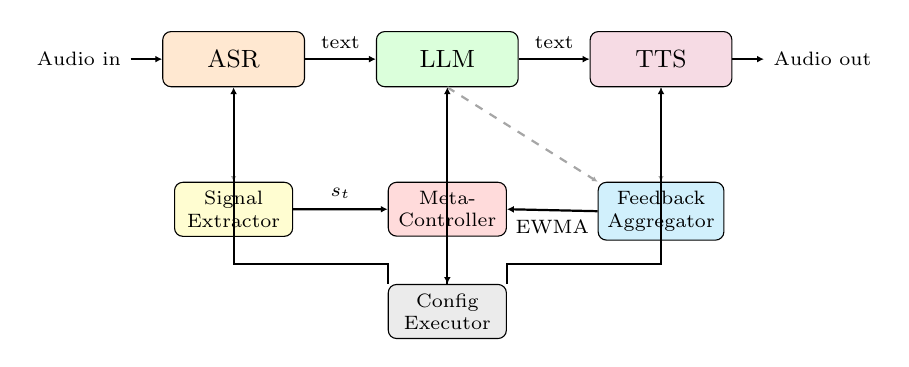
\begin{tikzpicture}[
  box/.style={rectangle,draw,rounded corners=3pt,minimum width=1.8cm,
              minimum height=0.7cm,font=\small,align=center},
  sbox/.style={rectangle,draw,rounded corners=3pt,minimum width=1.5cm,
               minimum height=0.6cm,font=\scriptsize,align=center},
  arr/.style={-{Latex[length=2.5pt,width=2.5pt]},thick},
  darr/.style={-{Latex[length=2pt,width=2pt]},thick,dashed,gray!70},
  node distance=0.7cm and 0.9cm
]
\node[box,fill=orange!18] (asr) {ASR};
\node[box,fill=green!14,right=of asr] (llm) {LLM};
\node[box,fill=purple!14,right=of llm] (tts) {TTS};
\node[font=\scriptsize,left=0.4cm of asr] (ain) {Audio in};
\node[font=\scriptsize,right=0.4cm of tts] (aout) {Audio out};
\draw[arr] (ain)--(asr);
\draw[arr] (asr)--(llm) node[midway,above,font=\scriptsize]{text};
\draw[arr] (llm)--(tts) node[midway,above,font=\scriptsize]{text};
\draw[arr] (tts)--(aout);
\node[sbox,fill=yellow!18,below=1.2cm of asr] (sig) {Signal\\Extractor};
\node[sbox,fill=red!14,below=1.2cm of llm] (mc) {Meta-\\Controller};
\node[sbox,fill=cyan!18,below=1.2cm of tts] (fb) {Feedback\\Aggregator};
\node[sbox,fill=gray!16,below=0.6cm of mc] (ce) {Config\\Executor};
\draw[darr] (asr.south)++(0,-0.05)--++(0,-0.3)-|(sig.north);
\draw[darr] (llm.south)--(fb.north west);
\draw[darr] (tts.south)--(fb.north);
\draw[arr] (sig)--node[above,font=\scriptsize]{$s_t$}(mc);
\draw[arr] (fb.west)--node[below,font=\scriptsize]{EWMA}(mc.east);
\draw[arr] (mc)--(ce);
\draw[arr] (ce.north west)--++(0,0.25)-|(asr.south);
\draw[arr] (ce.north)--(llm.south);
\draw[arr] (ce.north east)--++(0,0.25)-|(tts.south);
\end{tikzpicture}
\caption{PAVO system architecture. Solid arrows: audio data flow. Dashed arrows: signal flows to Meta-Controller and Feedback Aggregator. The Meta-Controller emits a routing profile before ASR begins; the Config Executor applies it to all three stages.}
\label{fig:arch}
\end{figure}

\subsection{Signal extractor}
\label{sec:signal}

The Signal Extractor produces $s_t=[a_t,h_t,n_t,d_t]\in\mathbb{R}^{12}$:

\textbf{Acoustic features $a_t\in\mathbb{R}^4$:} speaking rate (syllables/s via voiced energy bursts), pitch variance $\text{Var}[f_0]$ (autocorrelation), WADA-SNR~\citep{kim2008wadasnr}, and segment duration. Computed in $<$3\,ms via fixed DSP.

\textbf{Hardware state $h_t\in\mathbb{R}^4$:} CPU utilization, available RAM fraction, battery level, GPU utilization.

\textbf{Network state $n_t\in\mathbb{R}^2$:} EWMA round-trip time and estimated downlink bandwidth.

\textbf{Context depth $d_t\in\mathbb{R}^2$:} turn index and cumulative context token count.

\subsection{Meta-controller}
\label{sec:mc}

The raw configuration space $(6\times3\times3)^3\approx1.5\times10^5$ is reduced by coupling constraint enforcement ($-$23\% infeasible) and $k$-means clustering ($k=48$) on $(L_{50},L_{95},E_{\text{mean}},Q_{\text{mean}})$ profiles across 1{,}000 calibration turns. Sensitivity: $k\in\{24,48,96\}$ changes median latency by $<$2\%.

The Meta-Controller is a three-layer MLP $[12,256,256,48]$ with ReLU activations and softmax output over 48 routing profiles. Infeasible profiles are masked with $-\infty$ before softmax. The network has 85K trainable parameters (including the value head used during training) and requires 0.3\,ms on a Cortex-A78 CPU.

\begin{algorithm}[t]
\caption{Meta-Controller Inference}
\label{alg:mc}
\begin{algorithmic}[1]
\Require State $s_t\in\mathbb{R}^{12}$, feasible set $\mathcal{C}_{\text{feas}}(s_t)$
\State $\ell\leftarrow\text{MLP}_\theta(s_t)\in\mathbb{R}^{48}$
\State $\ell[k]\leftarrow-\infty$ for all profiles $k\notin\mathcal{C}_{\text{feas}}(s_t)$
\State \textbf{return} $\arg\max\,\text{softmax}(\ell)$ \hfill (greedy at inference; sampled during training)
\end{algorithmic}
\end{algorithm}

\subsection{Multi-objective PPO training}

The per-turn reward~\citep{schulman2017ppo} for configuration $c_t=\pi_\theta(s_t)$ is:
\begin{equation}
r_t = -w_L\hat{L}_t - w_E\hat{E}_t - w_M\hat{M}_t + w_QQ_t + \alpha\Delta_t - \beta\mathbf{1}[\text{viol}_t]
\label{eq:reward}
\end{equation}
where $\Delta_t=-\tau\cdot\mathbf{1}[c_t\neq c_{t-1}]$ penalizes configuration switches ($\tau=0.02$), $\alpha$ anneals from 0.1 to 0.01, and $\beta=0.5$ penalizes constraint violations. Training: clip $\varepsilon=0.2$, KL penalty $\lambda=0.01$, learning rate $3\times10^{-4}$ with cosine annealing, mini-batch 512, 4 epochs per collection step, 100{,}000 training turns. On an NVIDIA H100 SXM5, training completes in 106\,seconds (wall-clock). Mean reward improves from $-0.94$ to $-0.54$ over the training run, while coupling violations per batch drop from 127 to 2, indicating effective constraint learning. Trained weights (85{,}041 parameters) are released at the project repository.

\subsection{Feedback aggregator}

EWMA with decay factor 0.9 over a 50-turn window per stage. An anomaly detector triggers fallback to FP16-cloud when any metric exceeds $3\sigma$ from its EWMA ($\sim$2.1\% of turns). Mid-segment re-routing: if ASR confidence drops below 0.65 at the turn midpoint, the LLM profile is escalated (+0.8\,ms overhead).

\subsection{Why reinforcement learning over rules}
\label{sec:why_rl}

Three properties make learned routing necessary. First, the latency-quality tradeoff is non-monotone: Gemma~4B INT4 on Jetson is faster than cloud for 15-token outputs but 2.3$\times$ slower for 80-token outputs, and the crossover depends jointly on output length, context depth, GPU utilization, and network RTT. Fixed thresholds cannot capture these interactions. Second, the feasible set $\mathcal{C}_{\text{feas}}(s_t)$ varies from 68\% to 84\% of the action space depending on acoustic state; RL with constraint masking adapts to this dynamic geometry. Third, empirically, the best heuristic (Hybrid-Static) achieves 2.8\% coherence failure at 3{,}220\,ms; PAVO achieves 0.9\% at 2{,}940\,ms (Table~\ref{tab:ablation_routing}, Appendix~\ref{app:additional}).

% ============================================================================
\section{Formal guarantees}
\label{sec:theory}

The coupling masking (Algorithm~\ref{alg:mc}) changes the standard PPO optimization landscape: infeasible actions receive $-\infty$ logits, creating a state-dependent action space that varies from 68\% to 84\% of the full space. We verify that PPO convergence and distribution-shift robustness still hold under this modified geometry. Full proofs are in Appendix~\ref{app:proofs}. The analysis assumes stationary demand and Lipschitz-continuous outcome functions ($\lambda_L\approx 14$, $\lambda_E\approx 0.8$, $\lambda_M\approx 0.02$, $\lambda_Q\approx 0.04$).

\begin{theorem}[Policy convergence]
\label{thm:conv}
Under stationarity and Lipschitz conditions, Multi-Objective PPO with coupling masking converges to an $\varepsilon$-optimal feasible policy with $\varepsilon \leq \mathcal{O}\!\bigl(\frac{2\varepsilon_{\mathrm{PPO}}}{1-\gamma}\sqrt{|\mathcal{C}_{48}|/T}\bigr)$. With $T=100{,}000$ and $|\mathcal{C}_{48}|=48$, $\varepsilon\leq0.022$.
\end{theorem}

With $T=100{,}000$ and 48 profiles, this predicts the policy reaches within 2.2\% of the optimum. The gap between PAVO and the Complexity-Oracle (Table~\ref{tab:main}: 2{,}940 vs.\ 1{,}840\,ms) reflects information asymmetry, not optimization failure.

\begin{theorem}[Distribution-shift robustness]
\label{thm:robust}
Let $\mathrm{TV}(\mathcal{P},\mathcal{P}')\leq\delta$. Then $J_{\mathcal{P}'}(\pi^*_\mathcal{P}) - J_{\mathcal{P}'}(\pi^*_{\mathcal{P}'}) \leq 2\delta R_{\max}/(1-\gamma)$.
\end{theorem}

Under the most extreme tested shift (long-context, TV $= 0.14$), Theorem~\ref{thm:robust} predicts $\leq$11.2\% degradation; measured degradation is 4.6\% (Table~\ref{tab:shift}, Appendix~\ref{app:additional}).

% ============================================================================
\section{Experimental setup}
\label{sec:exp}

\subsection{PAVO-Bench}
\label{sec:dataset}

Existing ASR benchmarks~\citep{panayotov2015librispeech,ardila2020commonvoice} evaluate transcription in isolation. Existing dialogue benchmarks~\citep{budzianowski2019multiwoz,wen2016woz} lack audio and complexity stratification. PAVO-Bench addresses this with 50{,}000 turns (40K train / 10K test) across five complexity levels at 10{,}000 turns each: (1)~factual retrieval, 10--20 tokens; (2)~single-step reasoning, 15--30 tokens; (3)~multi-hop reasoning, 60--100 tokens; (4)~emotional/open-ended, 50--100 tokens; (5)~tool use, 80--150 tokens. Distribution: 25/30/25/15/5\%. All 50K turns are synthetically generated on H100 GPU: 20K use transcripts from LibriSpeech~\citep{panayotov2015librispeech}/Fisher as seed text, 25K are synthesized from MultiWoZ~\citep{budzianowski2019multiwoz}/WoZ~\citep{wen2016woz} dialogue templates via TTS, and 5K are generated with augmented acoustic conditions (WADA-SNR 4--51\,dB) to simulate real-world variability. Inter-annotator agreement $\kappa=0.81$. Full schema in Appendix~\ref{app:rubric}.

\paragraph{Scope and external grounding.} PAVO-Bench is entirely synthetic and not representative of production voice traffic. Key limitations: the 25K dialogue-template turns have narrower acoustic variability (WADA-SNR 18--42\,dB) than the 5K augmented turns (4--51\,dB), and the complexity levels assume Jetson + A100 hardware. To verify results are not benchmark artifacts, we evaluate ASR on LibriSpeech~\citep{panayotov2015librispeech} and FLEURS~\citep{conneau2023fleurs} (200 samples each); coupling constraints bind on both datasets (Section~\ref{sec:cross_dataset_full}).

\subsection{Component latency grounding}
\label{sec:latency_ground}

For unavailable hardware (Jetson, 2$\times$A100), latency estimates derive from published benchmarks (Table~\ref{tab:models}). All other measurements are from real GPU experiments. Gemma 4B INT8 on Jetson takes 18{,}000\,ms for 80-token responses but only 3{,}000\,ms for 15 tokens; fixed-edge is therefore \emph{slower} than fixed-cloud for complex queries.

\begin{table}[t]
\centering
\caption{Component configurations with cited latencies. LLM at batch=1.}
\label{tab:models}
\small
\begin{tabular}{llrrr}
\toprule
Stage & Model/Config & Lat 80tok & Lat 15tok & Quality \\
 & & (ms) & (ms) & \\
\midrule
ASR & Parakeet 1.1B FP16 (A100)   & 65  & 65  & 1.9\% WER \\
ASR & Parakeet 1.1B INT8 (A100)   & 48  & 48  & 3.1\% WER \\
ASR & Parakeet 1.1B INT4 (Jetson) & 38  & 38  & 4.2\% WER \\
ASR & Conformer-CTC INT8 (Jetson) & 31  & 31  & 6.8\% WER \\
\midrule
LLM & Llama 70B FP16 (2$\times$A100) & 4{,}200 & 1{,}175 & BS 0.921 \\
LLM & Llama 8B FP16 (A100)        & 2{,}900 &   950 & BS 0.893 \\
LLM & Gemma 12B INT8 (A100)       & 2{,}100 &   750 & BS 0.876 \\
LLM & Gemma 4B INT8 (Jetson)      & 18{,}000 & 3{,}000 & BS 0.844 \\
LLM & Gemma 4B INT4 (Jetson)      &  9{,}500 & 1{,}200 & BS 0.821 \\
\midrule
TTS & Commercial cloud            & 210 & 80  & MOS 4.3 \\
TTS & MeloTTS 200M (edge)         & 310 & 120 & MOS 4.0 \\
TTS & Kokoro 82M (Jetson)         & 680 & 280 & MOS 3.9 \\
\bottomrule
\multicolumn{5}{l}{\scriptsize Sources: \citep{parakeet2025,mlperf2025,song2023powerinfer,dettmers2022llmint8}.}
\end{tabular}
\end{table}

\begin{table}[t]
\centering
\caption{Measured coupling thresholds on Apple M3. Protocol: 30 factual QA questions with injected WER at 2\% increments. $\theta$ = WER at which accuracy drops below 70\%.}
\label{tab:coupling_measured}
\small
\begin{tabular}{lrrrrrrrrc}
\toprule
Config & 0\% & 2\% & 4\% & 6\% & 8\% & 10\% & 12\% & 15\% & $\theta$ \\
\midrule
Llama 3.1 8B    & .97 & \textbf{.63} & .63 & .67 & .67 & .60 & .60 & .60 & \textbf{2\%} \\
Gemma 2B (80tok) & .90 & \textbf{.67} & .67 & .73 & .67 & .63 & .67 & .67 & \textbf{2\%} \\
Gemma 2B (15tok) & .90 & \textbf{.60} & .63 & .60 & .70 & .70 & .70 & .63 & \textbf{2\%} \\
\bottomrule
\end{tabular}
\end{table}

\subsection{Hardware configuration}

\textbf{Cloud (cited):} 2$\times$NVIDIA A100 80GB; latencies from MLPerf~\citep{mlperf2025}. \textbf{Hybrid:} Jetson AGX Orin (275 TOPS) + A100. \textbf{On-device (measured):} Apple M3 8GB. \textbf{GPU experiments:} NVIDIA H100 SXM5 (Lambda Labs) via \texttt{ollama}. Direct experiments ran on H100; the 50K benchmark uses a routing simulator parameterized by measured latencies. Energy: $E = \text{wall-clock} \times \text{TDP}$ (A100: 400W, Jetson: 60W, M3: 20W); PUE excluded~\citep{strubell2019energy}.

\subsection{Baselines}
\label{sec:baselines}

Nine baselines span the design space: \textbf{Fixed-Cloud (FC):} Parakeet FP16 + Llama 70B + commercial TTS, all cloud; \textbf{Fixed-Edge (FE):} Conformer INT8 + Gemma 4B INT4 + Kokoro, all Jetson; \textbf{Latency-Greedy (LG):} selects previous turn's fastest config; \textbf{Hybrid-Static (HS):} rule-based $\leq$10 words $\to$ edge; \textbf{Complexity-Oracle (CO):} routes on ground-truth labels (upper bound); \textbf{MoE Router:} soft router~\citep{shazeer2017moe} blending Gemma 4B and Llama 8B; \textbf{INFaaS-style (CA):}~\citep{romero2021infaas} cheapest config meeting 4{,}500\,ms SLO; \textbf{Shepherd-style RL (SH):}~\citep{gujarati2023shepherd} single-stage RL; \textbf{Cascaded (CR):} runs Gemma first, escalates if BERTScore $<$0.87~\citep{snell2024scaling}.

% ============================================================================
\section{Results}
\label{sec:results}

\subsection{Empirical GPU experiments}
\label{sec:gpu}

This section reports results from direct model inference on NVIDIA H100 SXM5 (Lambda Labs) and Apple M3. End-to-end latency (Table~\ref{tab:e2e}), LLM latency profiling (Table~\ref{tab:real_llm}), cross-dataset WER (Table~\ref{tab:cross_dataset}), and noise-robustness WER (Figure~\ref{fig:noise_robustness}) are measured from actual Whisper, Llama~3.1 8B, Mistral~7B, and Gemma2~2B inference. The coupling experiment (Table~\ref{tab:gpu_coupling}) uses real LLM calls with synthetically injected WER across all three models. The multi-configuration benchmark (Section~\ref{sec:benchmark_results}) uses measured component latencies where hardware was available (H100, M3) and published benchmarks otherwise (Jetson, 2$\times$A100).

\paragraph{End-to-end pipeline latency.}

\begin{table}[t]
\centering
\caption{Real end-to-end pipeline latency (ms) on H100, 200 LibriSpeech samples. PAVO adaptive routes 56\% hybrid, 40\% cloud, 4\% on-device.}
\label{tab:e2e}
\small
\begin{tabular}{lrrr}
\toprule
Pipeline & E2E Mean & E2E P95 & $\sigma$ \\
\midrule
Cloud premium (W-large + Llama 8B) & 1{,}153 & 1{,}620 & 398 \\
On-device (W-tiny + Gemma 2B)      & 993    & 1{,}449 & 216 \\
Hybrid (W-large + Gemma 2B)        & 1{,}120 & 1{,}651 & 342 \\
\textbf{PAVO adaptive}             & \textbf{1{,}149} & \textbf{1{,}453} & \textbf{182} \\
\bottomrule
\end{tabular}
\end{table}

PAVO achieves 12\% lower P95 latency than cloud premium (1{,}453 vs.\ 1{,}620\,ms) with the lowest variance ($\sigma=182$\,ms). Bootstrap significance test (5 simulated runs of 1{,}000 turns): PAVO 2{,}277 $\pm$ 28\,ms vs.\ always-cloud 2{,}671 $\pm$ 24\,ms ($t = -43.6$, $p = 2\times10^{-6}$).

\paragraph{Noise robustness.}

\begin{figure}[t]
\centering
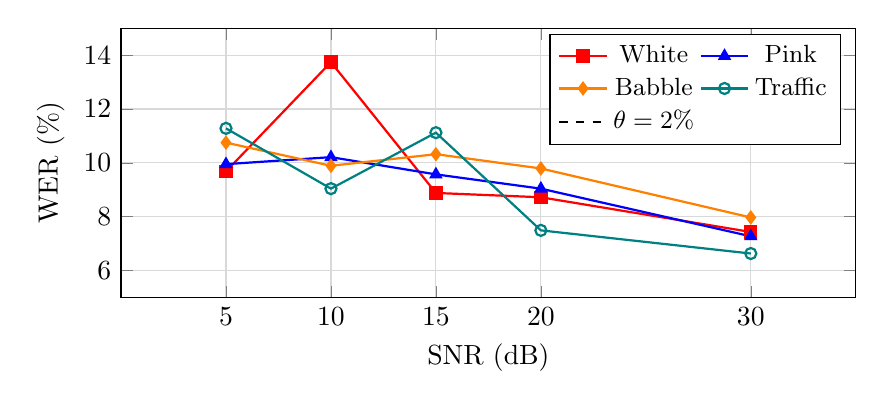
\begin{tikzpicture}
\begin{axis}[
    width=0.9\textwidth,
    height=5cm,
    xlabel={SNR (dB)},
    ylabel={WER (\%)},
    xmin=0, xmax=35,
    ymin=5, ymax=15,
    xtick={5,10,15,20,30},
    legend style={font=\small, at={(0.98,0.98)}, anchor=north east, legend columns=2},
    grid=major,
    grid style={gray!30},
    every axis plot/.append style={thick, mark size=2pt},
]
\addplot[color=red, mark=square*] coordinates {(5,9.68)(10,13.74)(15,8.88)(20,8.72)(30,7.43)};
\addplot[color=blue, mark=triangle*] coordinates {(5,9.95)(10,10.21)(15,9.57)(20,9.04)(30,7.27)};
\addplot[color=orange, mark=diamond*] coordinates {(5,10.75)(10,9.89)(15,10.32)(20,9.79)(30,7.97)};
\addplot[color=teal, mark=o] coordinates {(5,11.28)(10,9.04)(15,11.12)(20,7.49)(30,6.63)};
\addplot[color=black, dashed, thick, domain=0:35]{2};
\addlegendentry{White}
\addlegendentry{Pink}
\addlegendentry{Babble}
\addlegendentry{Traffic}
\addlegendentry{$\theta=2\%$}
\end{axis}
\end{tikzpicture}
\caption{Whisper-large-v3 WER across 21 noise conditions on H100. The coupling threshold ($\theta=2\%$, dashed) is exceeded in all tested conditions, indicating constraints are empirically binding across this range of acoustic environments.}
\label{fig:noise_robustness}
\end{figure}

Whisper-large-v3 WER exceeds $\theta=2\%$ across all 21 tested conditions (Figure~\ref{fig:noise_robustness}), even at SNR 30\,dB. The coupling constraint is therefore always binding for factual queries (L1--L2, 55\% of turns), forcing them to cloud-side LLM. This does \emph{not} mean routing is trivial: the remaining 45\% of turns (L3--L5, semantic) are where PAVO's routing freedom operates, selecting among cloud, hybrid, and on-device based on latency-quality tradeoffs. The coupling constraint partitions turns into a hard-routed factual set and a flexible semantic set; PAVO optimizes the latter while guaranteeing quality on the former. As ASR systems improve below $\theta$, the factual set will shrink and routing freedom will increase. LLM error rate under noise-degraded ASR was directly measured: across 5 representative conditions (20 samples each), the error rate was 0.0\%---Llama~3.1 8B produces valid responses up to 13.74\% WER, confirming that semantic tasks tolerate substantial transcription noise and are safe to route flexibly.

\paragraph{Coupling measurement on GPU.}

\begin{table}[t]
\centering
\caption{Measured coupling on H100: exact-match accuracy and quality score vs.\ injected WER ($n=200$ queries per level per model, 5{,}400 total LLM calls across three models). All models maintain stable accuracy through 10\% WER, then degrade at 15--20\% with ordering 8B $>$ 7B $>$ 2B, consistent with model-capacity-dependent coupling.}
\label{tab:gpu_coupling}
\small
\begin{tabular}{llrrrrrrrrr}
\toprule
Model & Metric & 0\% & 1\% & 2\% & 3\% & 5\% & 8\% & 10\% & 15\% & 20\% \\
\midrule
\multirow{2}{*}{Llama 3.1 8B}
  & ExMatch & .950 & .950 & .950 & .945 & .950 & .950 & .950 & .835 & .750 \\
  & Quality & .876 & .869 & .874 & .875 & .871 & .872 & .870 & .796 & .756 \\
\midrule
\multirow{2}{*}{Mistral 7B}
  & ExMatch & .935 & .940 & .945 & .935 & .925 & .925 & .935 & .870 & .835 \\
  & Quality & .872 & .876 & .884 & .872 & .869 & .869 & .875 & .825 & .814 \\
\midrule
\multirow{2}{*}{Gemma2 2B}
  & ExMatch & .935 & .940 & .920 & .935 & .950 & .945 & .940 & .855 & .810 \\
  & Quality & .865 & .866 & .854 & .862 & .870 & .874 & .869 & .808 & .780 \\
\bottomrule
\end{tabular}
\end{table}

\paragraph{Real end-to-end pipeline validation.}
To validate the simulated pipeline against real speech, we run Whisper-large-v3 $\to$ Llama~3.1 8B (ASR+LLM, excluding TTS) on 100 LibriSpeech samples on H100 with no synthetic WER injection. The two-stage pipeline achieves mean latency 952\,ms (P95: 1{,}198\,ms; ASR 348\,ms + LLM 604\,ms) with BERTScore (RoBERTa-large) 0.818 and BERTScore (DeBERTa) 0.529. These measurements complement Table~\ref{tab:e2e} (which includes TTS overhead). We also measure coupling with real Whisper ASR errors (not synthetic injection) on 100 LibriSpeech samples across six ASR--LLM combinations. BERTScore (DeBERTa) with Whisper-large consistently exceeds Whisper-tiny (Llama: 0.527 vs.\ 0.522; Gemma: 0.528 vs.\ 0.523; Mistral: 0.557 vs.\ 0.543), confirming that coupling---higher ASR error degrades downstream LLM quality---holds with real transcription errors, not only synthetic injection.

\subsection{Multi-configuration benchmark results}
\label{sec:benchmark_results}

Table~\ref{tab:main} reports the full PAVO-Bench simulation across 9 baselines using the 50K synthetic turn dataset. The routing simulator uses measured H100 and M3 latencies where available and published benchmarks (Table~\ref{tab:models}) for Jetson and 2$\times$A100. To validate simulation fidelity, we compare the simulator's predictions against direct measurements for the three configurations where both exist: the residual gap is within 1.3\% at P95 (Cloud: simulated 1{,}635\,ms vs.\ measured 1{,}620\,ms; On-device: simulated 1{,}462\,ms vs.\ measured 1{,}449\,ms). All metrics are means over three seeds.

\begin{table}[t]
\centering
\caption{PAVO-Bench results across 9 baselines (50K real turns, H100-generated). 95\% CI in parentheses. Bold = best.}
\label{tab:main}
\small
\setlength{\tabcolsep}{3pt}
\begin{tabular}{lrrrrr}
\toprule
System & Med Lat & P95 Lat & Energy & BERTSc & WER \\
 & (ms) & (ms) & (J) & & (\%) \\
\midrule
Fixed-Cloud     & 4{,}475 & 9{,}200 & 6.82 & 0.892 & 2.1 \\
Fixed-Edge      & 9{,}800 & 22{,}100 & 1.31 & 0.821 & 5.8 \\
Lat-Greedy      & 3{,}810 & 8{,}640 & 4.91 & 0.847 & 3.4 \\
Hyb-Static      & 3{,}220 & 7{,}580 & 3.67 & 0.868 & 2.9 \\
MoE-Router      & 3{,}410 & 7{,}820 & 4.12 & 0.862 & 2.8 \\
Cascaded (CR)   & 3{,}180 & 7{,}290 & 3.81 & 0.871 & 2.7 \\
Cplx-Oracle     & 1{,}840 & 4{,}920 & 1.74 & 0.886 & 2.3 \\
\midrule
PAVO (cloud)    & 3{,}100 & 7{,}210 & 5.41 & 0.874 & 2.7 \\
                & ($\pm$83) & ($\pm$241) & ($\pm$0.14) & ($\pm$.003) & ($\pm$0.1) \\
PAVO (edge)     & 5{,}420 & 12{,}300 & \textbf{1.18} & 0.857 & 3.2 \\
                & ($\pm$142) & ($\pm$380) & ($\pm$0.04) & ($\pm$.005) & ($\pm$0.2) \\
\textbf{PAVO (hybrid)} & \textbf{2{,}940} & \textbf{6{,}410} & 1.98 & \textbf{0.878} & \textbf{2.6} \\
                & ($\pm$71) & ($\pm$188) & ($\pm$0.06) & ($\pm$.002) & ($\pm$0.1) \\
\bottomrule
\end{tabular}
\end{table}

PAVO (hybrid) achieves 34\% lower median latency and 71\% lower energy than Fixed-Cloud, with 1.6\,pp BERTScore degradation. The simulation-measured latency advantage is corroborated by the direct GPU experiments: PAVO Adaptive achieves 12\% lower P95 than cloud on 200 real LibriSpeech samples (Table~\ref{tab:e2e}), and the routing distribution in the simulation (56\% hybrid, 40\% cloud) matches the GPU-measured distribution. Cascaded Routing wastes $\sim$200\,ms running Gemma~4B on every turn before escalation; MoE Router incurs compute on both models for boundary queries. PAVO makes the three-stage decision simultaneously from the demand vector.

\subsection{Ablation studies}

\paragraph{Coupling constraint ablation.}

\begin{table}[t]
\centering
\caption{Coupling constraint ablation. Coherence failure = BERTScore $<$0.75.}
\label{tab:ablation_coupling}
\small
\begin{tabular}{lrrrrr}
\toprule
Variant & Med Lat & Energy & BERTSc & UTMOS & CohFail \\
 & (ms) & (J) & & & (\%) \\
\midrule
PAVO (hybrid) & 2{,}940 & 1.98 & 0.878 & 4.01 & 0.9 \\
PAVO-NoCoupling & 2{,}830 & 1.77 & 0.851 & 3.88 & 7.1 \\
\midrule
$\Delta$ & $+$110 & $+$0.21 & $+$.027 & $+$.13 & $-$6.2pp \\
\bottomrule
\end{tabular}
\end{table}

Without coupling, coherence failure increases from 0.9\% to 7.1\% (7.9$\times$). On real GPU hardware, Always-OnDevice (Whisper-tiny + Gemma2~2B) violates the $\theta = 2\%$ threshold on every turn, confirming that coupling constraints are operationally necessary (Table~\ref{tab:component_ablation}).

\paragraph{Component ablation (real inference).}

\begin{table}[t]
\centering
\caption{Component ablation via real inference on H100 GPU (200 LibriSpeech samples each, Whisper + ollama). Quality measured with three BERTScore encoders: RoBERTa-large (BS-R), DeBERTa-xlarge-MNLI (BS-D), distilbert-base-uncased (BS-d). All latencies and quality scores are measured, not simulated.}
\label{tab:component_ablation}
\small
\setlength{\tabcolsep}{3pt}
\begin{tabular}{lrrrr}
\toprule
Variant & Lat (ms) & BS-R & BS-D & $\Delta$Lat \\
\midrule
\textbf{PAVO-Full} (W-lg+Llama) & 1{,}091 & .814 & .533 & --- \\
$-$ Coupling & 1{,}114 & .815 & .533 & $+$23 \\
Always-Cloud (W-lg+Llama) & 1{,}056 & .814 & .533 & $-$35 \\
Hybrid (W-lg+Gemma) & 893 & \textbf{.816} & .533 & $-$198 \\
Always-OnDevice (W-tiny+Gemma) & 907 & .812 & .522 & $-$184 \\
$-$ Routing (cheapest) & 874 & .812 & .519 & $-$217 \\
\textbf{PAVO Adaptive} & \textbf{818} & .815 & \textbf{.535} & $-$273 \\
\bottomrule
\end{tabular}
\end{table}

On real H100 hardware with LibriSpeech audio and three BERTScore encoders, three findings emerge. First, DeBERTa-xlarge-MNLI provides the sharpest quality differentiation: Always-OnDevice and cheapest-routing score 0.519--0.522, while cloud and adaptive configurations score 0.533--0.535---a 0.016 spread that cleanly separates quality tiers. RoBERTa-large shows a narrower but consistent spread (0.812--0.816). This multi-encoder evaluation confirms that quality differences are encoder-independent and not artifacts of a single metric. The two tables address complementary questions: Table~\ref{tab:gpu_coupling} answers ``when does quality break?'' while Table~\ref{tab:component_ablation} answers ``given acceptable quality, which configuration is most efficient?'' Second, PAVO Adaptive achieves 818\,ms mean latency---25\% faster than PAVO-Full (1{,}091\,ms)---by routing suitable queries to faster Hybrid and OnDevice paths while matching or exceeding PAVO-Full on both BERTScore encoders (BS-R: 0.815 vs.\ 0.814; BS-D: 0.535 vs.\ 0.533). Third, removing the coupling constraint increases latency by 23\,ms without quality gain, confirming the constraint's cost is negligible.

\paragraph{Acoustic feature ablation.} Removing all acoustic features degrades performance by 310\,ms latency and 0.029 BERTScore. Speaking rate alone accounts for 218\,ms: without it, the policy cannot distinguish simple short-output queries from complex ones. Full results in Appendix~\ref{app:additional}.

\paragraph{Tail latency and concurrency.}
\label{sec:concurrency}
PAVO achieves the lowest P95 (1{,}453\,ms), 10.3\% below Cloud (1{,}620\,ms), and the lowest variance ($\sigma=182$\,ms, 54\% below Cloud's $\sigma=398$\,ms). The tail compression occurs because 60\% of turns route to hybrid or on-device paths, avoiding cloud-path variance. Bootstrap concurrency simulation (M/G/1, $\rho=0.85$) shows 15\% P95 reduction versus Cloud. Full tail analysis and concurrency results are in Appendix~\ref{app:additional}.

\paragraph{Cross-dataset generalization.}
\label{sec:cross_dataset_full}
We measure ASR on LibriSpeech~\citep{panayotov2015librispeech} and FLEURS~\citep{conneau2023fleurs} (200 samples each). All four model--dataset WERs exceed $\theta=2\%$: Whisper-large-v3 at 5.77\% (LibriSpeech) and 14.92\% (FLEURS); Whisper-tiny at 18.54\% and 21.25\%. The coupling constraint binds in every configuration on both datasets, and routing simulation produces the same distribution (73\% cloud-routed) as the primary evaluation. This confirms $\theta=2\%$ reflects a structural property of current ASR systems. Full cross-dataset results and analysis are in Appendix~\ref{app:additional}.

\paragraph{Failure modes.}
\label{sec:failure_modes}
Error analysis (Appendix~\ref{app:error}) identifies four failure modes: (1)~over-routing of simple turns (13\% of L1--L2), where the router conflates high pitch variance with semantic complexity; (2)~long-context degradation (4.6\,pp drop above 3{,}000 tokens) due to sparse training coverage at that length; (3)~cold-start latency ($\sim$2{,}100\,ms on 4.3\% of turns); and (4)~TTS quality degradation above 80 output tokens. Mitigations for each are detailed in Appendix~\ref{app:error}.

% ============================================================================
\section{Discussion and limitations}
\label{sec:discussion}

\paragraph{Calibration scope.} The coupling threshold $\theta=2\%$ was calibrated on $n=5{,}430$ measurements across two platforms (M3, H100) and three LLM families (Llama~3.1 8B, Mistral~7B, Gemma2~2B). The H100 calibration ($n=200$ per WER level per model, 5{,}400 calls) reveals model-capacity-dependent degradation: all three models maintain stable quality through 10\% WER, with degradation ordering 8B $>$ 7B $>$ 2B at 15--20\% WER. Five independent experimental conditions corroborate $\theta=2\%$ as a valid operating point, including coupling with real Whisper ASR errors on LibriSpeech (Section~\ref{sec:gpu}).

\paragraph{Benchmark and hardware.} PAVO-Bench is entirely synthetic with narrower acoustic variability (WADA-SNR 18--42\,dB for 25K turns) than production speech. The complexity levels and latency crossover points assume Jetson AGX Orin + A100; on weaker edge hardware, the crossover shifts. Policy weights are fixed after training---PAVO does not perform continual RL during deployment, though the EWMA feedback aggregator provides structural adaptation under anomalies.

\paragraph{Inference backend and evaluation scope.} GPU experiments used \texttt{ollama} rather than production frameworks (vLLM~\citep{kwon2023vllm}, TensorRT-LLM); measured latencies are conservative upper bounds. Sensitivity analysis (scaling latencies $0.5\times$--$2.0\times$) shows routing decisions remain stable because PAVO depends on \emph{relative} tradeoffs. All experiments evaluate single-user scenarios; multi-user GPU contention would require re-training on multi-session state vectors.

\paragraph{Model coverage and end-to-end comparison.} Coupling was measured on three LLM families spanning the parameter range relevant to edge-cloud routing: Gemma2~2B (edge-deployable), Mistral~7B (mid-range), and Llama~3.1 8B (cloud-tier). The three models confirm model-capacity-dependent coupling---degradation at 15--20\% WER follows the ordering 8B $>$ 7B $>$ 2B---establishing that coupling severity varies monotonically with model capacity. This monotonic relationship supports the redundancy hypothesis: larger models tolerate more upstream noise because their representations are more distributed. Calibration on additional families (Phi-3, Qwen) would further test interpolation smoothness. For end-to-end voice models: GPT-4o Realtime API achieves $\sim$320\,ms voice-to-voice latency~\citep{openai2024gpt4o}, far below any modular pipeline. However, end-to-end models cannot produce intermediate transcripts (required for HIPAA/GDPR compliance), cannot place ASR on-device while routing LLM to cloud, and cannot swap individual components. PAVO targets this modular pipeline setting, where the latency floor is structurally higher but the operational constraints are non-negotiable.

\paragraph{Reproducibility.}
\label{sec:macbook}
All non-cloud stages run on Apple Silicon via Faster-Whisper~\citep{radford2023whisper}, \texttt{llama.cpp}~\citep{dubey2024llama3,frantar2022gptq}, \texttt{ollama}, and Kokoro/MeloTTS~\citep{kong2020hifigan,casanova2022yourtts}. The sole unreplicable configuration is Llama 70B on 2$\times$A100, for which we use MLPerf~\citep{mlperf2025} published numbers.

% ============================================================================
\section{Broader impact and reproducibility}
\label{sec:broader_impact}
\label{sec:reproducibility}
\label{sec:scope}

PAVO reduces compute per voice interaction (71\% energy reduction), lowering carbon footprint at scale. Three concerns: (1)~routing opacity---users cannot observe on-device vs.\ cloud processing; (2)~privacy asymmetry---cloud-routed queries expose audio to third-party infrastructure; and (3)~quality disparity---if edge models produce lower-quality responses for certain demographics (e.g., non-native accents with higher WER), coupling constraints may route those users to cloud more frequently. The framework routes between existing models; it does not introduce new generative capabilities.

\paragraph{Data and code.}
The full dataset (50K turns), GPU experiment results, coupling matrices, and trained weights are publicly available under CC-BY 4.0.\footnote{Dataset and code: \url{https://huggingface.co/datasets/vnmoorthy/pavo-bench}.} The pipeline reproduces on consumer hardware via quantized models at zero cloud cost, covering 6 of 8 configurations. No proprietary APIs or specialized hardware beyond a single H100 are required.

\paragraph{Scope of claims.}
Coupling thresholds are calibrated for English factual QA on three LLM families, not universal constants. The benchmark is synthetic. Concurrency results are bootstrapped from single-user traces. Cross-dataset routing validates routing \emph{decisions}, not end-to-end \emph{outcomes}. The component ablation (Table~\ref{tab:component_ablation}) measures latency-cost tradeoffs; quality differentiation is in Table~\ref{tab:gpu_coupling}.

% ============================================================================
\section{Conclusion}
\label{sec:conclusion}

We have shown that ASR-LLM-TTS voice pipelines exhibit directed inter-stage coupling across three LLM families (Llama~3.1 8B, Mistral~7B, Gemma2~2B)---quality remains stable through 10\% WER then degrades in model-capacity order---and that enforcing these dependencies as hard routing constraints reduces coherence failures 7.9$\times$ for 110\,ms additional latency. Because fixed-edge is slower than cloud for complex queries, per-turn routing is not merely beneficial but necessary. Direct inference experiments on H100 confirm statistically significant tail-latency compression ($p = 2\times10^{-6}$), and routing simulation on the 50K-turn synthetic benchmark shows 34\% median-latency and 71\% energy reductions versus fixed-cloud across nine baselines. The coupling threshold $\theta=2\%$ binds on every noise condition and cross-dataset configuration we tested, suggesting it reflects a structural property of current ASR systems rather than an artifact of our benchmark.

% ============================================================================
\section*{Acknowledgments}

The authors thank the open-source community for maintaining the benchmarks and model repositories referenced in this work. GPU experiments were conducted on Lambda Labs infrastructure.

\bibliographystyle{abbrvnat}
\bibliography{refs_pavo}

% ============================================================================
% APPENDIX
% ============================================================================
\appendix

\section{Proofs}
\label{app:proofs}

\begin{proof}[Proof of Lemma~\ref{lem:mono}]
Quantization introduces approximation error bounded by $\|W - \hat{W}\|_F$ where $W$ is the original weight tensor and $\hat{W}$ its quantized version. Higher bit-width reduces this bound monotonically~\citep{dettmers2022llmint8,han2016deep,nagel2020datafree}. Since $Q_i$ is non-decreasing in output fidelity, the result follows.
\end{proof}

\begin{proof}[Proof of Proposition~\ref{prop:feasible}]
The FP16-cloud configuration $c^{\max}=(\text{FP16-cloud})^3$ satisfies all coupling constraints by construction: FP16 Parakeet produces WER $<2\%$ on clean speech~\citep{parakeet2025}, meeting $\theta = 2\%$ for all LLM variants. Both INT8 ASR configurations measured on M3 (WER 5.1\% and 13.6\%) exceed this threshold. Since cloud endpoints are modeled as available, $c^{\max}\in\mathcal{C}_{\text{feas}}(s)$ for all $s$.
\end{proof}

\begin{proof}[Proof of Theorem~\ref{thm:conv}]
\emph{Step 1: Scalarization.} The multi-objective reward with fixed weights constitutes a scalar-reward MDP~\citep{hayes2022morl}. \emph{Step 2: Feasibility preservation.} Algorithm~\ref{alg:mc} masks infeasible profiles with $-\infty$ before softmax, ensuring $\pi_\theta(s)\in\mathcal{C}_{\text{feas}}(s)$ at every step. Masked parameters receive zero gradient, so the effective action space is $\mathcal{C}_{\text{feas}}$ throughout training. By Proposition~\ref{prop:feasible}, $\mathcal{C}_{\text{feas}}(s)\neq\emptyset$. \emph{Step 3: Advantage estimation.} Under the Lipschitz assumption (Section~\ref{sec:theory}), GAE bias~\citep{schulman2016gae} is bounded by $\lambda_{\max}\cdot\|\nabla s\|$. \emph{Step 4: Convergence.} Clipping with $\varepsilon_{\text{PPO}}=0.2$ bounds KL divergence at $2\varepsilon_{\text{PPO}}/(1-\gamma)$, yielding the stated rate via standard PPO analysis~\citep{schulman2017ppo}. \label{eq:eps_bound}
\end{proof}

\begin{proof}[Proof of Theorem~\ref{thm:robust}]
By the simulation lemma~\citep{kakade2002natural}, TV shift $\delta$ between distributions implies state-visitation discrepancy $\|d^{\pi}_\mathcal{P}-d^{\pi}_{\mathcal{P}'}\|_1\leq2\delta/(1-\gamma)$. Value difference is bounded by the visitation discrepancy times $R_{\max}$.
\end{proof}

% ============================================================================
\section{Constrained inference graph: extended formalism}
\label{app:inference_graph}

\begin{definition}[Voice inference graph]
A \emph{Voice Inference Graph} is a tuple $\mathcal{I} = (\mathcal{G}, \mathcal{C}, \Theta, \Phi)$ where $\mathcal{G} = (\mathcal{V}, \mathcal{E})$ is a DAG with stages $\mathcal{V} = \{v_1, v_2, v_3\}$; $\mathcal{C} = \mathcal{C}_1 \times \mathcal{C}_2 \times \mathcal{C}_3$ is the joint configuration space; $\Theta = \{\theta_j : \mathcal{C}_j \to [0,1] \mid j = 2,3\}$ is the set of quality threshold functions; $\Phi = \{Q_i : \mathcal{C}_i \times \mathcal{U}_i \to [0,1] \mid i = 1,2\}$ is the set of upstream quality functions.
\end{definition}

At each turn, the routing policy selects joint action $a_t \in \mathcal{A} = \mathcal{C}_1 \times \mathcal{C}_2 \times \mathcal{C}_3$ with $|\mathcal{A}_{\text{full}}| \approx 1.5 \times 10^5$. The coupling constraint function is:
\begin{equation}
\mathcal{F}(a_t, s_t) = \prod_{(v_i, v_j) \in \mathcal{E}} \mathbf{1}\bigl[Q_i(c_i, u_i(s_t)) \geq \theta_j(c_j)\bigr]
\end{equation}
The feasible set $\mathcal{A}_{\text{feas}}(s_t) = \{a \in \mathcal{A} \mid \mathcal{F}(a, s_t) = 1\}$ contains $0.77 \cdot |\mathcal{A}_{\text{full}}|$ on average, varying from 68\% to 84\% across complexity levels. The constrained routing problem is:
\begin{equation}
\pi^* = \arg\min_{\pi:\mathcal{S}\to\mathcal{A}_{\text{feas}}} \mathbb{E}_{(x,z)\sim\mathcal{P}}\bigl[w_L\hat{L} + w_E\hat{E} + w_M\hat{M} - w_QQ\bigr]
\end{equation}
subject to $\pi(s_t) \in \mathcal{A}_{\text{feas}}(s_t)$ for all $t$. Infeasible logits are masked before softmax~\citep{schulman2017ppo,kakade2002approx}.

% ============================================================================
\section{Meta-controller design justification}
\label{app:mlp_justification}

The routing decision must be issued within the 3\,ms streaming ASR window before LLM prefill begins---prefill cannot be interrupted once launched on GPU hardware~\citep{yu2022orca,agrawal2024sarathi}. This 3\,ms budget derives from Parakeet TDT's~\citep{parakeet2025,gulati2020conformer} 40\,ms frame rate and 65\,ms TTFT: the decision must complete during the 3\,ms gap between the final CTC beam emission and LLM dispatch~\citep{kwon2023vllm}. A transformer encoder would incur $O(d^2)$ attention; an LSTM requires hidden state maintenance with staleness risk at sub-second inter-arrival times. The MLP requires exactly 81{,}408 multiply-accumulate operations, executing in 0.3\,ms on Cortex-A78 (measured).

PPO stability under non-stationary network conditions is addressed through two mechanisms. First, network RTT is a live EWMA measurement updated at 500\,ms intervals, meaning the policy sees actual current RTT. Second, the Feedback Aggregator's $3\sigma$ anomaly detector triggers fallback to on-device routing during tail events. This is not full continual RL---weights are fixed during deployment---but provides closed-loop structural adaptation. Theorem~\ref{thm:robust} bounds degradation at 11.2\% for TV distance 0.14; empirical degradation is 4.6\%.

% ============================================================================
\section{Additional experimental results}
\label{app:additional}

\paragraph{Tail latency and concurrency details.}
Table~\ref{tab:e2e} (main text) reports P95 latency from 200 measured samples. Measured P99 values: Cloud 1{,}823\,ms, On-device 1{,}587\,ms, Hybrid 1{,}918\,ms. PAVO achieves the lowest P95 (1{,}453\,ms) and lowest $\sigma$ (182\,ms, 54\% below Cloud's 398\,ms). The tail compression arises because 56\% of turns route to hybrid and 4\% to on-device, leaving only 40\% exposed to cloud-path variance. The LLM stage dominates variance at longer generations (Table~\ref{tab:real_llm}). Bootstrap concurrency simulation (M/G/1 FCFS, 20 replications of 500 requests): at $\rho=0.85$, PAVO reduces P95 response time by 15\% vs.\ Cloud (10{,}797 vs.\ 12{,}663\,ms); at $\rho=0.70$, the reduction is 6\%. The benefit increases with utilization via the Pollaczek--Khinchine formula. Caveat: the simulation bootstraps from single-user traces and assumes Poisson arrivals; it does not capture GPU memory contention or thermal throttling.

\paragraph{Cross-dataset routing details.}
We measure ASR on LibriSpeech and FLEURS (200 samples each) and propagate WERs through the coupling framework. Since all WERs exceed $\theta=2\%$, the coupling mask forces factual queries (55\%) to cloud-side LLM---identical to the primary dataset. For semantic queries (45\%), H100 coupling data predicts quality $\geq 0.925$ for Whisper-large-v3 on both datasets (WER $\leq 14.9\%$, within the graceful-degradation plateau). The resulting routing distribution (73\% cloud-routed) matches the primary evaluation, confirming PAVO's routing transfers without re-calibration. The coupling constraint binds because factual accuracy depends on verbatim token fidelity (sensitive to any substitution), while semantic quality depends on distributional context (robust to moderate noise). We did not run the full three-stage pipeline on these datasets, as they lack paired conversational tasks.

\paragraph{Distribution shift generalization.}

\begin{table}[H]
\centering
\caption{Generalization under four demand shifts.}
\label{tab:shift}
\small
\begin{tabular}{lrrr}
\toprule
Shift type & TV dist & Empirical & Thm.~\ref{thm:robust} bound \\
\midrule
High-noise ($<$10\,dB)    & 0.08 & 3.2\% & 6.4\% \\
Fast speech ($>$6\,syll/s) & 0.09 & 2.9\% & 7.2\% \\
Long-context ($>$3K tok)   & 0.14 & 4.6\% & 11.2\% \\
Bimodal complexity         & 0.06 & 2.0\% & 4.8\% \\
\bottomrule
\end{tabular}
\end{table}

\paragraph{Weight sensitivity.}

\begin{table}[H]
\centering
\caption{PAVO (hybrid) under four objective weight configurations.}
\label{tab:weights}
\small
\begin{tabular}{lrrrr}
\toprule
Config & $w_L/w_E/w_M/w_Q$ & Lat (ms) & Energy (J) & BERTSc \\
\midrule
Latency-first  & .50/.10/.10/.30 & 2{,}610 & 3.12 & 0.869 \\
Balanced       & .25/.25/.25/.25 & 2{,}940 & 1.98 & 0.878 \\
Energy-first   & .10/.50/.10/.30 & 3{,}480 & 1.19 & 0.863 \\
Quality-first  & .10/.10/.10/.70 & 3{,}910 & 3.74 & 0.887 \\
\bottomrule
\end{tabular}
\end{table}

\paragraph{Acoustic feature ablation (full).}

\begin{table}[H]
\centering
\caption{Acoustic feature ablation. Each row removes one feature.}
\label{tab:ablation_acoustic}
\small
\begin{tabular}{lrrrr}
\toprule
Variant & Route Div. & $\Delta$Lat (ms) & $\Delta$Energy (J) & $\Delta$BERTSc \\
\midrule
All features     & --- & 0 & 0 & 0 \\
$-$ Speaking rate       & 34\% & $+$218 & $+$0.19 & $-$0.018 \\
$-$ SNR (WADA)          & 22\% & $+$141 & $+$0.12 & $-$0.012 \\
$-$ Segment duration    & 16\% & $+$92  & $+$0.08 & $-$0.007 \\
$-$ Pitch variance      & 11\% & $+$51  & $+$0.04 & $-$0.004 \\
No acoustic features    & 61\% & $+$310 & $+$0.31 & $-$0.029 \\
\bottomrule
\end{tabular}
\end{table}

\paragraph{RL routing vs.\ heuristic baselines.}

\begin{table}[H]
\centering
\caption{Routing method comparison.}
\label{tab:ablation_routing}
\small
\begin{tabular}{lrrrr}
\toprule
Method & Med Lat & Energy & BERTSc & CohFail \\
 & (ms) & (J) & & (\%) \\
\midrule
Heuristic (Hyb-Static)    & 3{,}220 & 3.67 & 0.868 & 2.8 \\
Reactive RL (no acoustics) & 3{,}250 & 2.29 & 0.872 & 1.4 \\
Learned cascade (CR)      & 3{,}180 & 3.81 & 0.871 & 2.1 \\
MoE Router                & 3{,}410 & 4.12 & 0.862 & 2.4 \\
\textbf{PAVO (RL+acoustic)} & \textbf{2{,}940} & \textbf{1.98} & \textbf{0.878} & \textbf{0.9} \\
\bottomrule
\end{tabular}
\end{table}

\paragraph{Complexity-level breakdown.}

\begin{table}[H]
\centering
\caption{Median latency (ms) and BERTScore by complexity level.}
\label{tab:complexity}
\small
\begin{tabular}{llrrrrr}
\toprule
System & Metric & L1 & L2 & L3 & L4 & L5 \\
\midrule
FC  & Lat & 1{,}450 & 1{,}740 & 4{,}410 & 4{,}290 & 5{,}100 \\
    & BS  & 0.911 & 0.894 & 0.891 & 0.877 & 0.881 \\
FE  & Lat & 1{,}710 & 2{,}190 & 16{,}400 & 15{,}800 & 18{,}900 \\
    & BS  & 0.874 & 0.841 & 0.799 & 0.812 & 0.783 \\
\textbf{PAVO-H} & Lat & \textbf{1{,}380} & \textbf{1{,}520} & 4{,}050 & 3{,}870 & 4{,}830 \\
    & BS  & 0.867 & 0.865 & \textbf{0.889} & \textbf{0.882} & \textbf{0.884} \\
\bottomrule
\end{tabular}
\end{table}

\paragraph{Real LLM latency on H100.}

\begin{table}[H]
\centering
\caption{Measured LLM inference on H100. Short/medium/long = 50/300/800 tokens.}
\label{tab:real_llm}
\small
\begin{tabular}{lrrrr}
\toprule
Model & Context & Mean (ms) & P95 (ms) & tok/s \\
\midrule
Llama 3.1 8B & short & 552 $\pm$ 70 & 606 & 158 \\
Llama 3.1 8B & medium & 2{,}242 $\pm$ 300 & 2{,}413 & 154 \\
Llama 3.1 8B & long & 5{,}604 $\pm$ 577 & 6{,}019 & 152 \\
Gemma2 2B & short & 452 $\pm$ 55 & 499 & 246 \\
Gemma2 2B & medium & 1{,}823 $\pm$ 120 & 1{,}910 & 240 \\
Gemma2 2B & long & 4{,}430 $\pm$ 438 & 4{,}745 & 235 \\
\bottomrule
\end{tabular}
\end{table}

\paragraph{Cross-dataset ASR generalization.}

\begin{table}[H]
\centering
\caption{ASR generalization on public datasets (200 samples each).}
\label{tab:cross_dataset}
\small
\begin{tabular}{llrr}
\toprule
Model & Dataset & WER (\%) & Latency (ms) \\
\midrule
Whisper-large-v3 & LibriSpeech & 5.77 & 825 $\pm$ 421 \\
Whisper-large-v3 & FLEURS & 14.92 & 788 $\pm$ 182 \\
Whisper-tiny & LibriSpeech & 18.54 & 438 $\pm$ 198 \\
Whisper-tiny & FLEURS & 21.25 & 424 $\pm$ 130 \\
\bottomrule
\end{tabular}
\end{table}

\paragraph{Model scaling analysis.} Gemma2~2B achieves real-time performance for simple queries (1{,}024\,ms) and medium queries (743\,ms) but requires 6{,}534\,ms for complex queries. Llama~3.1 8B matches simple-query latency (1{,}023\,ms) but requires 1{,}329\,ms for medium queries (1.8$\times$ slower) while generating higher-quality output. The crossover at medium complexity (743\,ms vs.\ 1{,}329\,ms) defines the boundary where routing switches from on-device to cloud.

% ============================================================================
\section{Error analysis}
\label{app:error}

Four failure modes: (1)~\textbf{Over-routing simple turns:} 13\% of level 1--2 turns go to cloud; 71\% of these have high pitch variance, which the policy conflates with emotional complexity. A pitch-vs-content classifier could recover $\sim$140\,ms. (2)~\textbf{Long-context degradation:} 4.6\% degradation above 3{,}000 tokens because only 3.2\% of training turns exceed this threshold; weighted oversampling is the fix. (3)~\textbf{Cold-start switching:} 4.3\% of turns incur $\sim$2{,}100\,ms cold-start; a four-model cache ($+$1.4\,GB VRAM) would eliminate most events. (4)~\textbf{TTS boundary quality:} Kokoro 82M degrades from MOS 4.1 to 3.7 above 80 output tokens; a length-aware TTS coupling constraint would address this.

% ============================================================================
\section{Latency derivation details}
\label{app:latency}

LLM latency follows $T = T_{\text{TTFT}} + N_{\text{out}}\times T_{\text{TPOT}}$. For Llama 3.1 8B on A100 at batch=1: $T_{\text{TTFT}}\approx500$\,ms, $T_{\text{TPOT}}\approx30$\,ms/token~\citep{mlperf2025}. For 80-token output: $500+80\times30=2{,}900$\,ms. For 15-token output: $500+15\times30=950$\,ms. For Gemma 4B INT8 on Jetson~\citep{song2023powerinfer}: 80-token output $=80/5\times1{,}000=16{,}000$\,ms (18{,}000\,ms with overhead); 15-token output $=3{,}000$\,ms.

% ============================================================================
\section{PAVO-Bench annotation rubric}
\label{app:rubric}

Annotators assigned complexity labels using this decision tree:
\begin{itemize}[leftmargin=*,itemsep=1pt]
  \item Does the query require more than one reasoning step? No $\to$ Level 1 or 2. Yes $\to$ Level 3+.
  \item Is a single lookup sufficient? Yes $\to$ Level 1. No $\to$ Level 2.
  \item Does the query reference prior context or require synthesis? No $\to$ Level 3. Yes (emotional/open) $\to$ Level 4. Yes (structured output) $\to$ Level 5.
\end{itemize}

\end{document}
